\section{Fundamentação Matemática}

\subsection{Redes Neurais}

% ---------------------------------------------------------------- 14
\begin{frame}{Formulação Matemática de Redes Neurais}
  Composição de transformações afins separadas por ativações não lineares,
  ajustada por erro quadrático médio.
  \begin{columns}[T]
    \column{0.44\textwidth}
      \vspace{-4pt}
      \begin{align*}
        h^{(0)} &= x, \\
        h^{(l)} &= \sigma\!\left(W^{(l)} h^{(l-1)} + b^{(l)}\right), \\
        u_\theta(x) &= W^{(L)} h^{(L-1)} + b^{(L)}.
      \end{align*}
    \column{0.52\textwidth}
      \begin{center}
        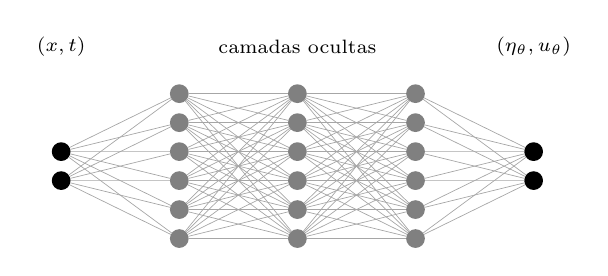
\begin{tikzpicture}[
            xscale=0.60, yscale=0.46,
            nnnode/.style={circle, draw, line width=0.5pt, minimum size=0.22cm, inner sep=0pt},
            inout/.style={nnnode, fill=black, draw=black},
            hidden/.style={nnnode, fill=gray, draw=gray},
            conn/.style={draw=gray!70, line width=0.25pt}
          ]
          \node[inout] (x1) at (0,-2.4) {};
          \node[inout] (x2) at (0,-3.2) {};
          \node[font=\scriptsize] at (0,0.5) {$(x,t)$};
          \foreach \i in {1,...,6} { \node[hidden] (h1_\i) at (2.5,-0.8*\i) {}; }
          \foreach \i in {1,...,6} { \node[hidden] (h2_\i) at (5.0,-0.8*\i) {}; }
          \node[font=\scriptsize] at (5.0,0.5) {camadas ocultas};
          \foreach \i in {1,...,6} { \node[hidden] (h3_\i) at (7.5,-0.8*\i) {}; }
          \node[inout] (out1) at (10.0,-2.4) {};
          \node[inout] (out2) at (10.0,-3.2) {};
          \node[font=\scriptsize] at (10.0,0.5) {$(\eta_\theta, u_\theta)$};
          \foreach \j in {1,...,6} {
            \draw[conn] (x1) -- (h1_\j);
            \draw[conn] (x2) -- (h1_\j);
          }
          \foreach \i in {1,...,6} {
            \foreach \j in {1,...,6} {
              \draw[conn] (h1_\i) -- (h2_\j);
              \draw[conn] (h2_\i) -- (h3_\j);
            }
          }
          \foreach \i in {1,...,6} {
            \draw[conn] (h3_\i) -- (out1);
            \draw[conn] (h3_\i) -- (out2);
          }
        \end{tikzpicture}
      \end{center}
  \end{columns}
  \begin{itemize}[<+->]
    \item $\theta = \{W^{(l)}, b^{(l)}\}$: parâmetros treináveis;
    \item $\sigma$ sigmoidal aplicada elemento a elemento;
    \item Função de perda padrão contra um conjunto de dados
          $\mathcal{S} = \{(x_i, u_i)\}_{i=1}^N$:
          \[
            \mathcal{L}(\theta) = \frac{1}{N}\sum_i \|u_\theta(x_i) - u_i\|^2 .
          \]
  \end{itemize}
\end{frame}

% ---------------------------------------------------------------- 17
\begin{frame}{Formulação Matemática de PINNs}
  A PINN \parencite{raissi2019} insere a EDP na otimização: além dos dados, a rede
  é forçada a satisfazer as equações.
  \begin{equation*}
    \mathcal{L}_{\text{PINN}}(\theta)
      = \underbrace{\frac{1}{N_\mathcal{D}}\sum_{i} \bigl\| \mathcal{D}[u_\theta](x_i,t_i) \bigr\|^2}_{\text{resíduo da EDP}}
      + \underbrace{\frac{1}{N_0}\sum_{i} \bigl\| u_\theta(x_i,0) - u_0(x_i) \bigr\|^2}_{\text{condição inicial}} .
  \end{equation*}
  Para o sistema de Boussinesq, $\mathcal{D}$ é o par de resíduos
  \begin{align*}
    \mathcal{D}_1 &= (\eta_\theta)_t + (u_\theta)_x + \alpha\,(\eta_\theta u_\theta)_x, \\
    \mathcal{D}_2 &= (u_\theta)_t - \tfrac{\beta}{3}(u_\theta)_{xxt} + (\eta_\theta)_x + \alpha\,u_\theta (u_\theta)_x .
  \end{align*}
  \begin{itemize}[<+->]
    \item Derivadas por diferenciação automática
          \parencite{linnainmaa1970, paszke2019pytorch}; Adam \parencite{kingma2014adam};
    \item $(\alpha,\beta)$ fixados, uma PINN aprende para só um par, mas há implementações que aprendem como apenas mais um canal de features.
  \end{itemize}
\end{frame}

\subsection{Operadores Neurais}

% ---------------------------------------------------------------- 18
\begin{frame}{Formulação Matemática de Operadores Neurais}
  \setlength{\abovedisplayskip}{4pt}\setlength{\belowdisplayskip}{4pt}%
  Sejam $\mathcal{A}$ e $\mathcal{U}$ espaços de Banach de funções sobre $D$. O alvo é o
  operador solução $G^\dagger : \mathcal{A} \to \mathcal{U}$, remodelamos o problema como o mapeamento $(\alpha, \beta) \mapsto (\eta, u)$. Um operador neural o aproxima por
  \begin{equation*}
    G_\theta = Q \circ \sigma\bigl(W_L + \mathcal{K}_L\bigr) \circ \cdots \circ
               \sigma\bigl(W_1 + \mathcal{K}_1\bigr) \circ P ,
  \end{equation*}
  em que cada camada atualiza os canais por
  \begin{equation*}
    v_{\ell+1}(x) = \sigma\Bigl((W_\ell\,v_\ell)(x) + (\mathcal{K}_\ell v_\ell)(x)\Bigr).
  \end{equation*}
  \begin{itemize}[<+->]
    \item $P : \mathbb{R}^{d_a} \to \mathbb{R}^{d_c}$: operador de elevação, leva a
          entrada ponto a ponto a $d_c \gg d_a$ canais;
    \item $W_\ell$: mapa linear local; $\sigma$: ativação aplicada ponto a ponto;
    \item $\mathcal{K}_\ell$: operador integral não local, com kernel aprendido
          $\kappa_\ell : D \times D \to \mathbb{R}^{d_c \times d_c}$, que faz cada ponto
          da saída ler a função inteira:
          \[
            (\mathcal{K}_\ell v)(x) = \int_D \kappa_\ell(x,y)\,v(y)\,dy ;
          \]
    \item $Q : \mathbb{R}^{d_c} \to \mathbb{R}^{d_u}$: projeção de volta à dimensão da
          saída;
    \item Cada parametrização de $\kappa_\ell$ dá uma arquitetura.
  \end{itemize}
\end{frame}

% ---------------------------------------------------------------- 19
\begin{frame}{Formulação Matemática de FNOs}
  % três equações em destaque: espaçamento vertical reduzido só neste frame
  \setlength{\abovedisplayskip}{4pt}\setlength{\belowdisplayskip}{4pt}%
  O FNO \parencite{li2021} toma o kernel invariante por translação,
  $\kappa_\ell(x,y) = \kappa_\ell(x-y)$.
  O operador $\mathcal{K}_\ell$ é uma convolução de $\kappa_\ell$ com $v_\ell$, então
  \begin{equation*}
    (\mathcal{K}_\ell v_\ell)(x) = \int_D \kappa_\ell(x-y)\,v_\ell(y)\,dy.
  \end{equation*}
  \uncover<2->{%
  Isto é,
  \begin{equation*}
    (\mathcal{K}_\ell v_\ell)(x)
      = \mathcal{F}^{-1}\Bigl(\mathcal{F}(\kappa_\ell)\cdot\mathcal{F}(v_\ell)\Bigr)(x).
  \end{equation*}}%
  \begin{itemize}
    \item<3-> Coeficientes de Fourier do kernel são matrizes treináveis $R_{\ell,k}$ truncadas em $|k| \le k_{\max}$;
    \item<4-> Invariância à discretização, mas mantendo padrão para FFTs de $2^N$ pontos.
  \end{itemize}
  \uncover<5->{%
  Treino puramente supervisionado, com $(\eta_\theta^i, u_\theta^i) = G_\theta(\alpha_i, \beta_i)$:
  \begin{equation*}
    \mathcal{L}_{\text{FNO}}(\theta) = \frac{1}{M}\sum_{i=1}^{M}\frac{1}{N_x N_t}\sum_{j=0}^{N_x-1}\sum_{n=0}^{N_t}
    \Bigl[\bigl(\eta_\theta^i(x_j,t_n) - \eta_i(x_j,t_n)\bigr)^2
    + \bigl(u_\theta^i(x_j,t_n) - u_i(x_j,t_n)\bigr)^2\Bigr].
  \end{equation*}}
\end{frame}

% ---------------------------------------------------------------- 20
\begin{frame}{Formulação Matemática de PINOs}
  O PINO \parencite{li2023pino} mantém o esqueleto do FNO e soma resíduo e condição
  inicial ao termo de dados:
  \begin{equation*}
    \mathcal{L}_{\text{PINO}}(\theta)
      = \lambda_{\text{pde}}\,\mathcal{L}_{\text{pde}}(\theta)
      + \lambda_{\text{ic}}\,\mathcal{L}_{\text{ic}}(\theta)
      + \lambda_{\text{data}}\,\mathcal{L}_{\text{data}}(\theta).
  \end{equation*}
  \begin{itemize}[<+->]
    \item Para o sistema de Boussinesq, a saída são duas matrizes $N_x \times N_t$ da aproximação de $\eta$ e $u$ em um único forward pass para um dado $\alpha=\beta$ qualquer (é input também);
    
    \item Avaliar o resíduo da EDP é diferenciar numericamente essa matriz, não a rede;
  
    \item Derivadas espaciais pseudoespectrais e temporais por diferenças finitas (Euler implícito, seguindo implementação original de \textcite{li2023pino}) \parencite{li2023pino_code};
    
    \item Permite aproveitar conhecimento das equações.
  \end{itemize}
\end{frame}

\subsection{Viés Espectral e Neural Tangent Kernel}

% ---------------------------------------------------------------- 15
\begin{frame}{Viés espectral: estudo via fluxo do gradiente}
  A descida do gradiente com taxa de aprendizado $\mu > 0$ atualiza os parâmetros por
  \begin{equation*}
    \theta^{(k+1)} = \theta^{(k)} - \mu\,\nabla_\theta\mathcal{L}(\theta^{(k)})
    \quad\Longleftrightarrow\quad
    \frac{\theta^{(k+1)} - \theta^{(k)}}{\mu} = -\nabla_\theta\mathcal{L}(\theta^{(k)}).
  \end{equation*}
  \uncover<2->{%
  Lendo os iterados como amostras de uma curva $\theta(\tau)$ nos instantes
  $\tau^{(k)} = k\mu$, o lado esquerdo vira um quociente de diferenças progressivas:
  \begin{equation*}
    \frac{\theta(\tau^{(k)} + \mu) - \theta(\tau^{(k)})}{\mu}
      = -\nabla_\theta\mathcal{L}\bigl(\theta(\tau^{(k)})\bigr).
  \end{equation*}}%
  \uncover<3->{%
  Com $\mu \to 0$, chegamos à EDO do fluxo do gradiente:
  \begin{equation*}
    \frac{d\theta}{d\tau} = -\nabla_\theta\mathcal{L}(\theta), \qquad \theta(0) = \theta^{(0)}.
  \end{equation*}}%
  \uncover<4->{%
  A descida do gradiente é exatamente o método de Euler explícito aplicado a essa EDO,
  com passo $\mu$ \parencite{suli2003, burden2011}.}
\end{frame}

% ---------------------------------------------------------------- 15b
\begin{frame}{Viés espectral: Neural Tangent Kernel}
  Com $e(\tau) = \bigl(u_\theta(x_i) - u_i\bigr)_{i=1}^{N}$ o vetor de erros pontuais e
  $J(\theta) = \partial e/\partial\theta$ seu Jacobiano, após algumas manipulações do fluxo
  do gradiente, considerando a regra da cadeia\footnote{Ver Seção~2.3.3 do texto do TCC.},
  chegamos a
  \begin{equation*}
    \frac{de}{d\tau} = -J(\theta)\,J(\theta)^{T}\,e(\tau)
    \quad\Longrightarrow\quad
    \frac{de}{d\tau} = -K(\theta)\,e(\tau),
    \quad\text{onde}\quad
    K_{ij}(\theta) = \nabla_\theta e_i^{T}\,\nabla_\theta e_j .
  \end{equation*}
  \uncover<2->{%
  $K(\theta)$ é o NTK empírico \parencite{jacot2018}: a matriz de Gram do
  produto interno dos gradientes.}
\end{frame}

% ---------------------------------------------------------------- 15c
\begin{frame}{Viés espectral: NTK quase constante}
  Em redes largas, cada parâmetro se move pouco durante o treino, e o Jacobiano quase
  não muda: $K(\theta(\tau)) \approx K_0$ \parencite{jacot2018, chizat2019}.
  \begin{center}
    
\includegraphics[width=0.92\linewidth,clip,trim=0 97 0 15]{wangntk.png}\\[2pt]
    {\scriptsize\color{black!55}Variação relativa (a) dos parâmetros $\theta$ e (b) do
     NTK $K$ de uma PINN para Poisson 1D; (c) autovalores do NTK na inicialização e ao fim do treino
     \parencite{wang2022ntk}.}
  \end{center}
  Assim,
  \[
    \frac{de}{d\tau} = -K\bigl(\theta\bigr)\,e\bigl(\theta\bigr)
      \approx -K\bigl(\theta(\tau_0)\bigr)\,e(\tau),
  \]
  obtendo uma EDO linear com coeficientes constantes para evolução do vetor de erros.
\end{frame}

% ---------------------------------------------------------------- 16
\begin{frame}{Viés espectral: EDO da evolução do erro}
  Com o kernel parado na inicialização, o erro segue $\dfrac{de}{d\tau} = -K_0\,e(\tau)$.
  Como $K_0$ é simétrica e semidefinida positiva \parencite{strang2006, golub2013},
  \begin{equation*}
    K_0 = V\Lambda V^{T}, \qquad V^{T}V = I, \qquad
    \Lambda = \mathrm{diag}(\lambda_1,\ldots,\lambda_N), \quad
    \lambda_1 \ge \cdots \ge \lambda_N \ge 0 .
  \end{equation*}
  \uncover<2->{%
  Mudando de base, $c(\tau) = V^{T}e(\tau)$ e $e(\tau) = V c(\tau)$:
  \begin{equation*}
    \frac{dc}{d\tau} = -\Lambda\,c(\tau).
  \end{equation*}}%
  \uncover<3->{%
  Como $\Lambda$ é diagonal, o sistema se desacopla em $N$ EDOs escalares:
  \begin{equation*}
    \frac{dc_k}{d\tau} = -\lambda_k\,c_k(\tau)
    \quad\Longrightarrow\quad
    c_k(\tau) = c_k(0)\,e^{-\lambda_k\tau}, \qquad k = 1,\ldots,N.
  \end{equation*}}
\end{frame}

% ---------------------------------------------------------------- 16b
\begin{frame}{Viés espectral: solução do sistema desacoplado}
  Voltando à base original, obtemos a solução completa da EDO
  $\dfrac{de}{d\tau} = -K_0\,e(\tau)$:
  \begin{equation*}
    e(\tau) = \sum_{k=1}^{N} \bigl(v_k^{T} e_0\bigr)\, e^{-{\color{AmurmapleRed}\lambda_k} \tau}\, v_k .
  \end{equation*}
  \uncover<2->{%
  Autovetores com $\lambda_k$ grande somem rápido; os de $\lambda_k$ pequeno persistem
  por todo o treino \parencite{cao2019}.}
\end{frame}

% ---------------------------------------------------------------- 16c
\begin{frame}{Viés espectral: base de Fourier e comparação direta}
  Se os dados estão numa grade regular e a função alvo é periódica, o erro admite a
  DFT. Com a matriz de Fourier unitária $F$ ($F^{*}F = I$), $\hat{e}(\tau) = F\,e(\tau)$ e
  \begin{equation*}
    \frac{d\hat{e}}{d\tau} = F\,\frac{de}{d\tau} = -F K_0 F^{-1}\,\hat{e}(\tau),
    \qquad
    F K_0 F^{-1} = (FV)\,\Lambda\,(FV)^{-1}.
  \end{equation*}
  \uncover<2->{%
  As colunas $F v_k$ diagonalizam a dinâmica. Com $\tilde{c}(\tau) = (FV)^{-1}\hat{e}(\tau)$,
  os mesmos passos dão $\tilde{c}_k(\tau) = \tilde{c}_k(0)\,e^{-\lambda_k\tau}$ e
  \begin{equation*}
    \hat{e}(\tau) = \sum_{k=1}^{N} \bigl[(F v_k)^{*}\hat{e}_0\bigr]\, e^{-{\color{AmurmapleRed}\lambda_k}\tau}\,(F v_k).
  \end{equation*}}%
  \uncover<3->{%
  Os autovetores de maior $\lambda_k$ são suaves e concentrados nas baixas frequências
  \parencite{rahaman2019, xu2019frequency}: o conteúdo de baixa frequência do erro
  decai primeiro.}
\end{frame}

% ---------------------------------------------------------------- 16d
\begin{frame}{Viés espectral: iterações por frequência}
  Se quisermos garantir que o erro na $k$-ésima componente seja menor que
  $\varepsilon > 0$, podemos isolar:
  \begin{equation*}
    |v_k^{T} e(0)|\,e^{-\lambda_k\tau} < \varepsilon
    \quad\Longrightarrow\quad
    \tau > \frac{1}{\lambda_k}\,\ln\frac{|v_k^{T} e(0)|}{\varepsilon}.
  \end{equation*}
  \uncover<2->{%
  Mas esta estimativa é em $\tau$; fazendo a mesma análise para a versão discretizada,
  chegamos em:
  \begin{equation*}
    |v_k^{T} e(0)|\,|1 - \mu\lambda_k|^n < \varepsilon
    \quad\Longrightarrow\quad
    n > \frac{1}{-\ln|1 - \mu\lambda_k|}\,\ln\frac{|v_k^{T} e(0)|}{\varepsilon}.
  \end{equation*}}%
  \uncover<3->{%
  Aproveitando, como o método do gradiente aqui nada mais é do que o método de Euler
  explícito, a taxa de aprendizado (tamanho do passo) segue as mesmas estimativas que
  garantem a estabilidade do método, ou seja, $\mu < 2/\lambda_{\max}$
  \parencite{suli2003, leveque2007}; tomamos assim $\mu = 0{,}4/\lambda_{\max}$.}
\end{frame}
